\documentclass[10pt]{beamer}

%PTBR
%\usepackage[brazilian]{babel}
\usepackage[utf8]{inputenc}
\usepackage[T1]{fontenc}
\usepackage{bm}
\usepackage{graphicx}
\usepackage[absolute,overlay]{textpos} %pacote para posicionar o logo na primeira página
%\usepackage[dvipsnames]{xcolor}

%\usepackage{enumitem}

\usetheme[progressbar=frametitle]{metropolis}
\usepackage{appendixnumberbeamer}

\usepackage{booktabs}
\usepackage[scale=2]{ccicons}

\usepackage{pgfplots}
\usepgfplotslibrary{dateplot}

\usepackage{xspace}
\newcommand{\themename}{\textbf{\textsc{metropolis}}\xspace}

\newcommand{\induceint}{\ensuremath{\Imc_{\Amc^{*}, \Tmc}}}
\newcommand{\fullminmod}{\ensuremath{\Imc_{\Amc^{*}, \Tmc}} \cup \Imc_{\min}(\Tmc)}

\usepackage{Macros}

%\definecolor{teal}{rgb}{0.0, 0.5, 0.5}
%\definecolor{darkorange}{rgb}{1.0, 0.55, 0.0}

\title{Rational Instance Checking in Defeasible \ELIbot}

\titlegraphic{%
  \begin{picture}(0,0)
    \put(305,-120){\makebox(0,0)[rt]{
\includegraphics[width=6cm]{img/logos.png}}}
  \end{picture}}

\date{\today}
\author{Igor de Camargo e Souza Câmara}
\institute{University of São Paulo}

\begin{document}

\begin{frame}[plain]
  \titlepage
\end{frame}

\begin{frame}[fragile]{Challenge 1}

\begin{align*}
  & \Amc = \{a:C, b:C, (a, b):r\} \\
  & \Tmc = \{D \sqcap \exists r.D \sqsubseteq \bot \} \\
  & \Dmc = \{C \definc D\}
\end{align*}

\pause

\begin{center}
  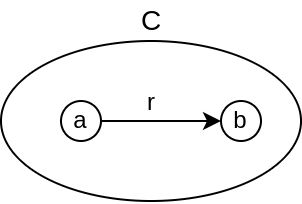
\includegraphics[scale=0.5]{img/challenge1_1.png}
  \end{center}

\end{frame}

\begin{frame}[fragile]{Challenge 1}

\begin{center}
  $\Tmc = \{D \sqcap \exists r.D \sqsubseteq \bot \}$
\end{center}

\pause

(\textbf{Solution no. 1} -- Apply $C \definc D$ to $a$)

\begin{center}
  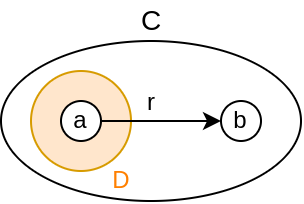
\includegraphics[scale=0.35]{img/challenge1_2.png}
\end{center}
  
\pause
\vspace{0.2cm}

(\textbf{Solution no. 2} -- Apply $C \definc D$ to $b$)

\begin{center}
  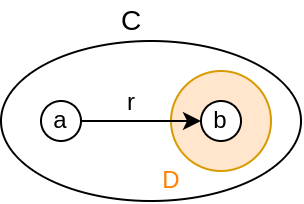
\includegraphics[scale=0.35]{img/challenge1_3.png}
\end{center}

\end{frame}

\begin{frame}{Solution no.1 [Casini \& Straccia, 2010]}
  
  $\models$ defined \wrt an order $s$ over the individuals in $\Kmc$.

  \pause
  \vspace{0.7cm}

  $s = (a, b)$ characterizes the first solution, \ie 

  $\Kmc \models_s D(a) \text{ and } \Kmc \not \models_s D(b)$

  \vspace{0.7cm}

  $s' = (b, a)$ characterizes the first solution, \ie 

  $\Kmc \models_{s'} D(b) \text{ and } \Kmc \not \models_s D(a)$

\end{frame}

\begin{frame}{Adapting C\&S method to typicality model semantics}

{\large
  Procedure defined in Pensel \& Turhan (2018)
}

{\large
  \begin{enumerate}
    \item Enrich $\Amc$ with defeasible information respecting an order $s$. The result is denoted by $\Amc^{*}$. \pause
    \item $\Amc^{*}$ and $\Tmc$ induce an interpretation $\Imc_{\Amc^{*}, \Tmc}$. \pause 
    \item $\Imc_{\Amc^{*}, \Tmc}$ is quasi-disjoint \wrt minimal typicality model $\Imc_{\min}(\Tmc)$. \pause
    \item Define the new minimal typicality model as $\Imc_{\Amc^{*}, \Tmc} \cup \Imc_{\min}(\Tmc)$. 
  \end{enumerate}
}
\end{frame}

\begin{frame}{Adapting C\&S method to typicality model semantics}

  Inducing an interpretration from $\Amc^{*}$ and $\Tmc$

  \vspace{0.5cm}

    Let $\Kmc = (\Amc, \Tmc)$. Then $\Aint = (\Delta^{\Aint}, \cdot^{\Aint})$ s.t.:
    
    \begin{align*}
        & \Delta^{\Aint} = \sig{\Amc} \cup Qc(\Kmc) \text{ where } Qc(\Kmc) \text{ denotes quantified concepts in }\Kmc. \\
        & a^{\Aint} = a \\
        & A^{\Aint} = \{a \in \sig{\Amc} : \Kmc \models A(a) \} \\ 
        & r^{\Aint} = \{r(a,b) \in \Amc \} \cup \{(a, \typel{E}{\emptyset}) : \Kmc \models (\exists r.E)(a)\}
    \end{align*}

\end{frame}

\begin{frame}{Adapting C\&S method to typicality model semantics -- Example}

$\Amc = \{a:C, b:C, (a, b):r \}$ 

$\Tmc = \{ D \sqcap \exists r.D \sqsubseteq \bot \}$

$\Dmc = \{ C \definc D \}$

$s = (a, b)$

\pause
\vspace{0.3cm}

$\Amc^{*} = \{a:C, {\color{red} a:D}, b:C, (a, b):r\}$

\pause
\vspace{0.3cm}

$\induceint$

$\Delta^{\induceint} = \{a, b\}$

$C^{\induceint} = \{a, b\}$

$D^{\induceint} = \{a\}$

$r^{\induceint} = \{(a,b)\}$
\end{frame}

\begin{frame}{Remarks}
\begin{enumerate}
  \item $\fullminmod$ is a canonical model \wrt materialization-based rational reasoning, \pause
  \item Individuals affect the upgrade procedure.
\end{enumerate}

\pause
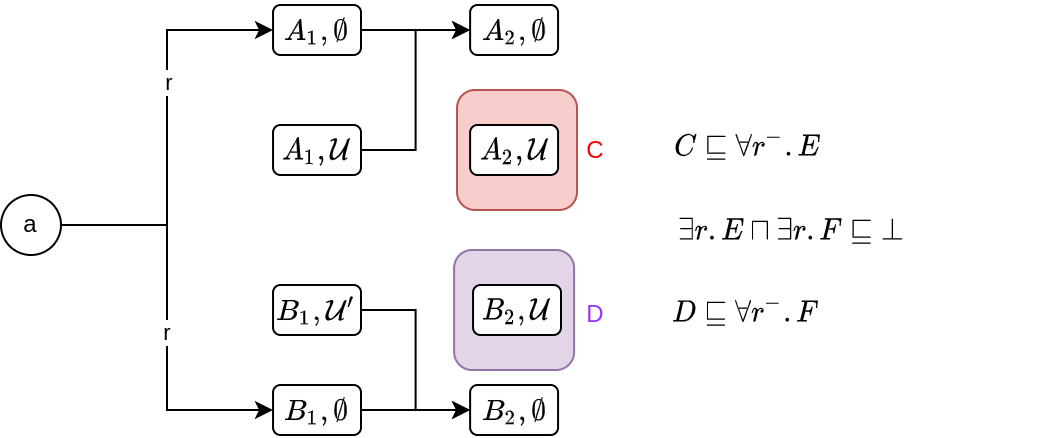
\includegraphics[scale=0.35]{img/indblockcon1.png}

\end{frame}

\begin{frame}{Remarks}
  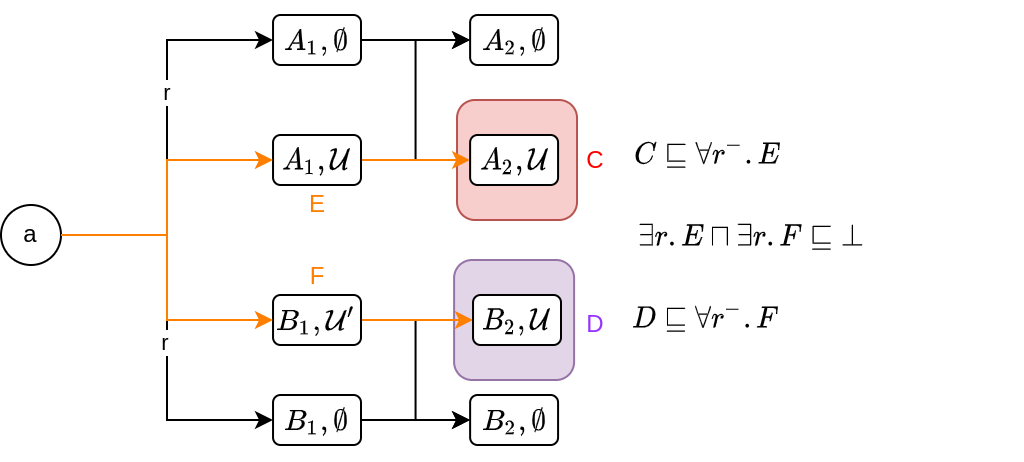
\includegraphics[scale=0.37]{img/indblockcon2.png}
\end{frame}

\begin{frame}{What happens with defeasible \ELIbot}

Quasi-disjointness in \ELbot

\begin{quote}
  (Definition) $\Jmc$ is quasi-disjoint from $\Imc$ iff 
  \begin{itemize}
    \item $\forall A\in \Cname$, $A^{\Jmc} \cap \Delta^{\Imc} = \emptyset$ and 
    \item $\forall r \in \Rname $, $r^{\Jmc} \cap (\Delta^{\Imc} \times (\Delta^{\Imc} \cup \Delta^{\Jmc})) = \emptyset$
  \end{itemize}
\end{quote}

\begin{center}
  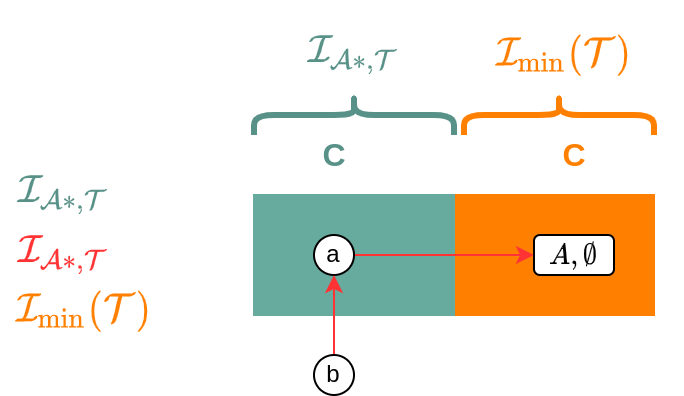
\includegraphics[scale=0.3]{img/quasid.png}
\end{center}

\end{frame}

\begin{frame}{What happens with defeasible \ELIbot}

The following property holds for \ELbot

\begin{quote}
  For $\Imc, \Jmc$ \st $\Jmc$ is quasi-disjoint from $\Imc$ it holds that $C^{\Imc \cup \Jmc} \cap \Delta^{\Imc} = C^{\Imc}$
  For all \ELbot concepts $C$
\end{quote}

\pause
... but not in \ELIbot 

$\Jmc$ s.t. $\Delta^\Jmc = \{ a, C \}$, $r^\Jmc = \{(a,C)\}$ and $(\exists r^{-}.\top)^{\Jmc} = \{ C\}$

$\Imc$ s.t. $\Delta^{\Imc} = \{ C \}$, $r^{\Imc} = \emptyset$ and $(\exists r^{-}.\top)^{\Jmc} = \emptyset$.

\end{frame}

\begin{frame}{Without quasi-disjointness...}
\begin{definition}[New ABox Interpretation]
    \label{def:abint}
    Let $\Kmc = (\Amc, \Tmc)$. Then:
    \begin{align*}
        & \Delta^{\Aint}  = \sig{\Amc} \cup {\color{red} \{\typel{M}{\emptyset} : M \in \Pmc (\sig{\Tmc})\}} \\
        & a^{\Aint} = a \\
        & A^{\Aint} = \{a \in \sig{\Amc} : \Kmc \models A(a) \}  \\ 
        & r^{\Aint} = \{r(a,b) \in \Amc \} \\ 
        & \cup {\color{red}\{(a, \typel{M}{\emptyset}) : \Kmc \models (\exists r.\setconj{M})(a) \textrm{ and $M$ is maximal for $\Kmc, r$ and $a$}\}} \\ & \cup {\color{red}\{(\typel{M}{\emptyset}, a) : \Kmc \models (\exists r^-.\setconj{M})(a) \textrm{ and $M$ is maximal for $\Kmc, r^{-}$ and $a$}\}}
    \end{align*}
\end{definition}
\end{frame}

\begin{frame}{Why the new construction do NOT break the model property}

  \[ A \sqsubseteq B \mid A \sqsubseteq \exists r.B \mid A \sqsubseteq \forall r.B\]

\vspace{0.5cm}

  {\begin{center}
  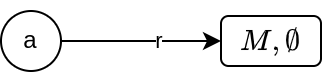
\includegraphics[scale=0.37]{img/simple.png}
  \end{center}}

  \pause 
  \vspace{0.5cm}

  With the new definition 

  \begin{itemize}
    \item $\fullminmod \models \Kmc$.
    \item $\fullminmod$ is \emph{canonical} \wrt rational defeasible subsumption and defeasible instance checking (for named concepts).
  \end{itemize}

  % No nominals + Maximality

\end{frame}

\begin{frame}{Upgrading the typicality of the edges}

  { \Large 
  \begin{enumerate}
    \item Upgrades of edges owned by individuals can block upgrades of concept representatives. \pause
    \item Individuals own every edge to which they belong. \pause
    \item There are three types of violations brought by upgrades on edges with individuals.
\end{enumerate}
  }
\end{frame}

\begin{frame}{Violation \#1}
  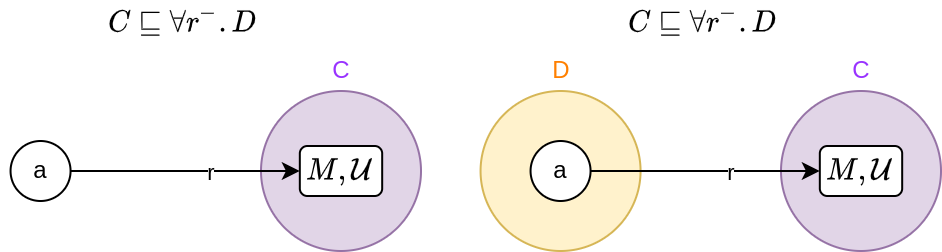
\includegraphics[scale=0.33]{img/repair_incon.png}
\end{frame}

\begin{frame}{Violation \#2}
  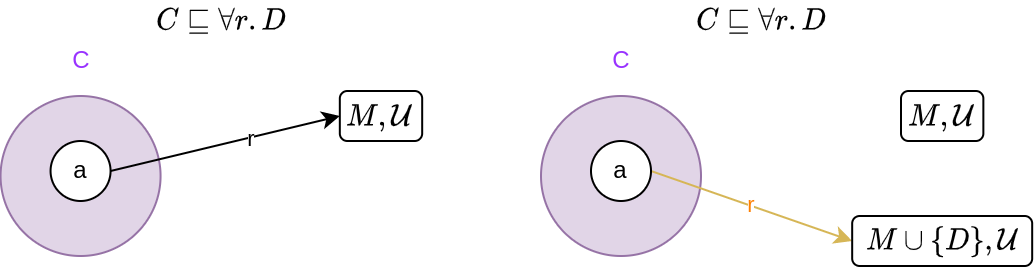
\includegraphics[scale=0.3]{img/repair_conin.png}
\end{frame}

\begin{frame}{Violation \#3}
  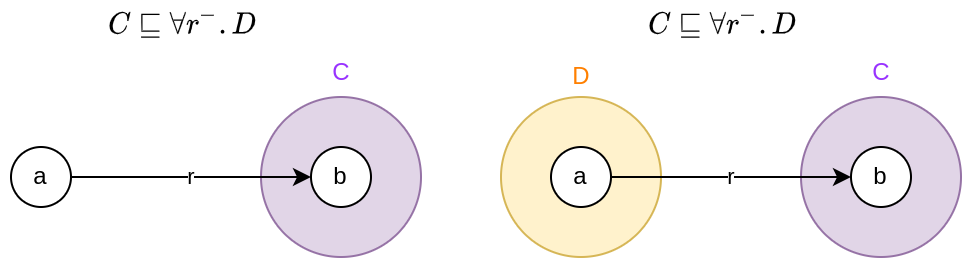
\includegraphics[scale=0.33]{img/repair_inin.png}
\end{frame}

\begin{frame}{Quantification Neglect and Defeasible Instance Checking}
  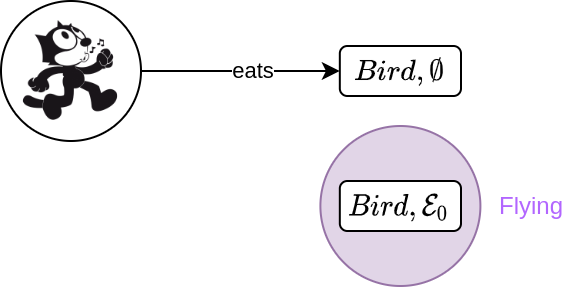
\includegraphics[scale=0.5]{img/propex_felix.png}
\end{frame}

\begin{frame}{Quantification Neglect and Defeasible Instance Checking}
  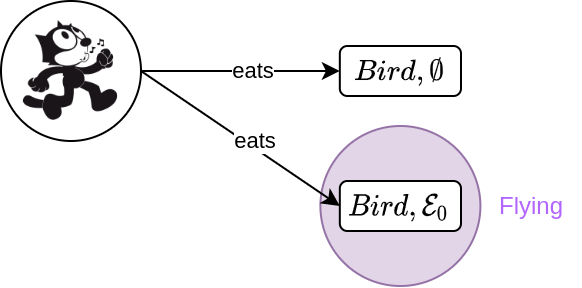
\includegraphics[scale=0.5]{img/nestex_felix.png}

\vspace{0.5cm}

\begin{center}
  {\Large 
  $ \Kmc \modelsnest{rat} (\exists \dlFont{eats}.\dlFont{Flying})(\dlFont{felix})$
  }
\end{center}

\end{frame}

\begin{frame}{Next chapters}
  \begin{itemize}
    \item Instance checking in relevant and lexicographic defeasible reasoning.
    \item Skeptical instance checking without order over individuals.
    \item Defeasible assertions?
  \end{itemize}
\end{frame}

\end{document}




